%Latex2e file
\documentclass[12pt,letterpaper]{article}
%\renewcommand{\arraystretch}{2}
%\input{\scrload.tex}
\setlength{\textwidth}{6.5in}
\setlength{\textheight}{9.5in}

\setlength{\oddsidemargin}{-.25in}
\setlength{\evensidemargin}{-.25in}
\setlength{\topmargin}{-.25in}
\pagestyle{empty}

\usepackage{amsmath}
\usepackage{amssymb}
\usepackage{graphicx}

\newcommand{\R}{\ensuremath{{\mathbb{R}}}}
\newcommand{\Z}{\ensuremath{{\mathbb{Z}}}}
\newcommand{\Q}{\ensuremath{{\mathbb{Q}}}}
\newcommand{\N}{\ensuremath{{\mathbb{N}}}}
\newcommand{\C}{\ensuremath{{\mathbb{C}}}}
\newcommand{\Proof}{\noindent {\bf Proof: }}
\newcommand{\QED}{\begin{flushright}QED\end{flushright}}
\newcommand{\Refl}{{\bf Reflexive: }}
\newcommand{\Symm}{{\bf Symmetric: }}
\newcommand{\Tran}{{\bf Transitive: }}
\newcommand{\ep}{\varepsilon}
\newcommand{\ri}{\right|}
\newcommand{\lef}{\left|}
\newcommand{\toR}{\to \R}
\newcommand{\fancy}[1]{#1_{\text{fancy}}}
\newcommand{\pro}[1]{\noindent {\bf #1}}
\newcommand{\prob}[1]{\newpage\noindent {\bf #1}}
\newcommand{\bacon}{\approx}

   
\begin{document}
\begin{flushright}
Nick Kerner
Homework 1
\end{flushright}
\begin{center}
\large{Geometry}\\
\end{center}

 HISTORICAL EXERCISE SET.
1. As indicated earlier, Egyptian geometers used the formula A = (1/4)(a + c)(b + d) to calculate the area of any quadrilateral whose successive sides have lengths a, b, c, and d.
(a) Does this formula work for squares? For rectangles that are not squares?\\

This formula can be rewritten $\frac{a + c}{2} \frac{b+d}{2}$.  Since in both rectangles (AAHH) and squares opposite sides have the same length we know that $\frac{a + c}{2} \frac{b+d}{2} = \frac{2a}{2}\frac{2b}{2} = ab$ where a and b are lengths of perpendicular sides.  This is the modern formula for calculating the area of squares and rectangles, and yes, it does work.\\

(b) If you choose specific lengths for the sides of an isosceles trapezoid, how does the result compare to the actual area? Repeat for two other isosceles trapezoids. Do the same for three specific parallelograms.\\

An isosceles trapezoid has two same-length legs while the other two sides are opposite and parallel. Let us call the legs a and c while the other sides are b and d.  So the formula the Egyptians used was $\frac{a + c}{2} \frac{b+d}{2} = \frac{2a}{2}\frac{b+d}{2} = a\frac{b+d}{2}$.\\

Isosceles 1:
Let a = 2, b = 3, c = 1.  According to their formula, the area is $2\frac{1+3}{2} = 4$. The actual area is calculated by dissecting the trapezoid into 3 separate sections, two right triangles with the legs of the trapezoid as their hypotenuses and a rectangle between them.  First we know that the base and summit of the rectangle have length c, so there is length 2 left for legs of the right triangles.  This gives these triangles legs of length 1 and $\sqrt{3}$ as determined by the Pythagorean theorem. This gives the rectangle height $\sqrt{3}$ and therefore area $1(\sqrt{3})$ and each triangle will have area $\frac{\sqrt{3}}{2}$ Therefore the total area of the trapezoid is $\frac{\sqrt{3}}{2} + \frac{\sqrt{3}}{2} + \sqrt{3} = 2\sqrt{3}$ which is irrational and most certainly not equal to 4.\\

Isosceles 2: Let a=5, b=7, c=1.  According to their formula the area is $5\frac{1+7}{2} = 20$.  Once again breaking the trapezoid into 2 right triangles and a rectangle we get a rectangle height (and triangle leg length) of 4.  This gives the rectangle area 4 (its other side is c which has length 1) and the right triangle areas will add to 12 (each having area $6 = 3\frac{4}{2}$).  This gives the total isosceles area to be $16\neq 20$.\\

Isosceles 3:  Let a=5, b=9, c=3.  According to their formula the area is $5\frac{9+3}{2} =30$.  Once again breaking the trapezoid into 2 right triangles and a rectangle we get a rectangle height of 4.  This gives the rectangle area 12 (c=3 is a side of the rectangle) and the right triangle areas will add to 12 (each having area $6 = 3\frac{4}{2}$).  This gives the total isosceles area to be $24\neq 30$.\\

\newpage 

Note that in the case of parallelograms, the Egyptian formula reduces to $a\frac{b+c}{2} = a\frac{b+b}{2} = a\frac{2b}{2} = ab$.

Parallelogram 1:
Let a=1, b=$\sqrt{2}$ and let one pair of opposite angles be 45 degree angles.  Note that since opposite sides are of the same length, the Egyptian formula reduces to $ab$.  Additionally, this cuts precisely into two right triangles each with hypotenuse $\sqrt{2}$ and legs length 1.  This means that this parallelogram has area 1 (as each triangle has area .5), while the Egyptian formula would assign it area $\sqrt{2}$. \\

Parallelogram 2:
Let a=2, b=$\sqrt{2}$ and let one pair of opposite angles be 45 degree angles  Additionally, this cuts precisely into a rectangle with length 1 and two right triangles each with hypotenuse $\sqrt{2}$ and legs length 1.  The triangles again have area $.5$ each and the height of the rectangle, which is also a leg of the triangles is 1.  Therefore the parallelogram has area 1.  This means that this parallelogram has area 2 (as each triangle has area .5 and the square has area 1), while the Egyptian formula would assign it area $2\sqrt{2}$. \\


Parallelogram 3:
Let a=$4$, b=$5$ and let one pair of opposite angles be 45 degree angles.  Additionally, this cuts precisely into a rectangle with length 1 and two right triangles each with hypotenuse $5$ and each with a leg length 3.  The triangles again have area $6$ (Pythagorean triple triangle sides 3,4, and 5 thus area 6) each and the height of the rectangle, which is also a leg of the triangles is 4.  Therefore the rectangle has area 4.  This means that this parallelogram has area 16 (as each triangle has area 6 and the rectangle has area 4), while the Egyptian formula would assign it area $20$. \\

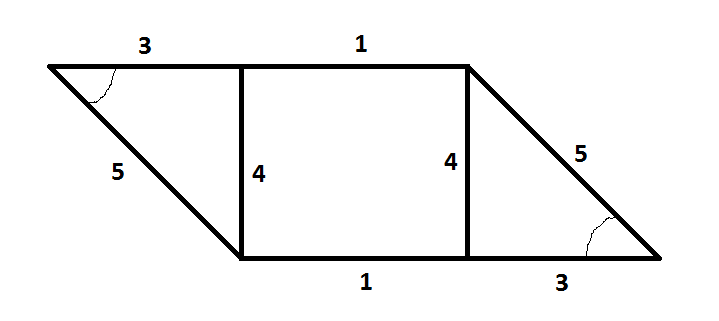
\includegraphics[width=2.5in]{parallelogram3.png}



\newpage 
(c) Generalize your results for part (b).


The Egyptian formula for the area of a isosceles trapezoid gives an area that is too large unless the isosceles trapezoid is a rectangle.  A formula for the area of the trapezoid would be the average of the opposite sides of different length (base and summit as opposed to the legs) times the height of the interior rectangle ($h\frac{b + d}{2}$, where the isosceles pair of sides have length $a=c$, $h = \sqrt{a^2 - \left( \frac{\lef b - d\ri}{2}\right)^2}$).  The Egyptian formula can be written as the product of the averages of opposite sides, which shares a part with the other formula I have provided.  Since the legs have the same length, the part of the product that they produce is an overestimate of the height except in the case where the trapezoid is a rectangle. Therefore 

\begin{eqnarray*}
h &=& \sqrt{a^2 - \frac{\lef b - d\ri}{2}}\\
&=& \sqrt{a^2 - \left(\frac{\lef b - d\ri}{2}\right)^2}\text{ since $\frac{\lef b - d\ri}{2}$ is a leg of a triangle with hypotenuse $a$}\\
&\leq& \sqrt{a^2}\\
&=& a
\end{eqnarray*}

so $A = h\frac{b + d}{2} \leq a\frac{b+d}{2}$ since $h \leq a$. \\



The Egyptian formula for the area of a parallelogram would only work if it is indeed a rectangle.  As you change the angles on the parallelogram, the area decreases but the Egyptian formula does not show this.  This can be demonstrated by reducing a pair of opposite angles from 90 to 0.  As this happens, adjacent sides come closer to becoming a straight line (when the angle between them reaches 0).  When this happens, the area of the parallelogram reaches 0.  Therefore the area of the parallelogram according to the Egyptians is always greater than or equal to our modern calculations.






\newpage 

2. If a and b are the lengths of the legs of a right triangle and c is the length of the hypotenuse, Babylonian geometers approximated the length of the hypotenuse by the formula $c = b + (a^ 2/2b).$\\

(a) How does this approximation compare to the actual result when a = 3 and b = 4? When a = 5 and b = 12? When a = 12 and b = 5?\\

Case 1: a = 3, b = 4.  When these are the legs this forms a Pythagorean triple with c= 5.  Using the Babylonian formula, we get $c= 4 + (9/8) = 5.125$.  The actual hypotenuse is 5 showing that this is an overestimation.\\

Case 2: a = 5 and b = 12 .  These legs form a Pythagorean triple with c = 13. Using the Babylonian formula yields $c = 12 + (25/24) = 13 + (1/24)$\\

Case 3: a = 12 and b = 5.  These legs again form the Pythagorean triple with c = 13.  Using the formula we get c= 5 + 144/10 = 19.4 which is severe overestimation.\\

(b) Give an algebraic argument demonstrating that this formula results in an approximation that is too large.\\

First we know that the formula is actually $a^2 + b^2 = c^2$, so if we show that $c^2 > a^2 + b^2$ under the Babylonian formula then $c > \sqrt{a^2 + b^2}$ which means our Babylonian approximation is too large.  Starting with the Babylonian formula, 

\begin{eqnarray*}
c &=& b + (a^ 2/2b)\\
&=&  \frac{2b^2 + a^2}{2b}\\
c^2 &=& \frac{4b^4 + 4a^2b^2 + a^4}{4b^2}\\
&=& a^2 + b^2 + \frac{a^4}{4b^2} \\
&>& a^2 + b^2 \text{ as } \frac{a^4}{4b^2} > 0
\end{eqnarray*}

\newpage 

3. The following was translated from a Babylonian tablet created about 2600 B.C. Explain what it means.\\

60 is the circumference, 2 is the perpendicular, find the chord. Double 2 and get 4, do you see?
Take 4 from 20 and get 16. Square 20, and you get 400. Square 16, and you get 256. Take 256
from 400 and you get 144. Find the square root of 144. 12, the square root, is the chord. This
is the procedure.\\

This is the formula to obtain the `chord'.  If you draw a line tangent to the circle (of circumference 60) and draw a perpendicular segment (call it AT) of length 2 into the circle at the point where the tangent line intersects the circle (call this point T), the chord is the line segment connecting two points on the circle together with point A parallel with the original tangent line (perpendicular to AT).  AT can also be constructed by drawing it along a diameter with one endpoint on the circle.

This can be demonstrated in the following way.  First, draw a circle and the perpendicular of length two inward into the circle.  Then draw the chord (this algorithm is to find the chord's length, but we can draw it ahead of time).  Now take a copy of the circle and rotate it 180 degrees on itself.  Because this rotation is around the center of the circle, if we connect a point on the circle with the rotated version of itself, it will connect through the center of rotation, therefore this line segment will be a diameter of the circle.  Take one endpoint of the chord and connect it with the rotated version of itself, say for segment BC connect B to B'.  Then connect B' to C.  The segment BB' is a diameter of the circle and B'C is two lengths of the perpendicular less than the diameter (clearly visible in a diagram).  This gives us a right triangle as the chord and the rotated chord are parallel.  Using the Pythagorean theorem we can now find the length of a chord. 

\begin{center}
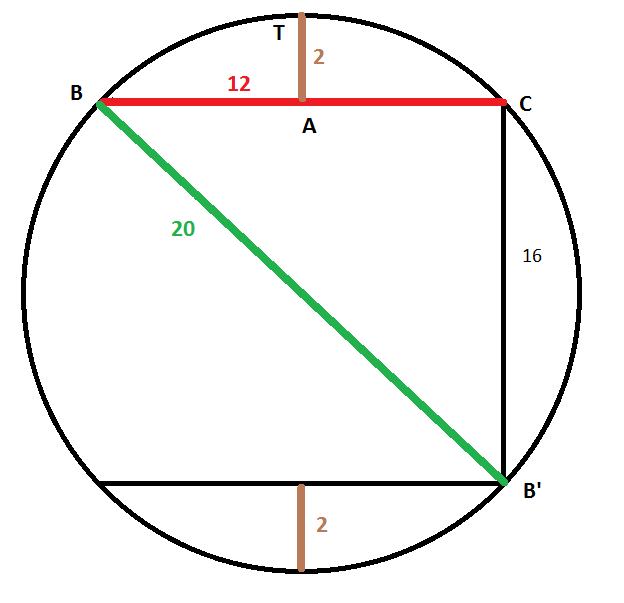
\includegraphics[width=3in]{circle.png}
\end{center}

\newpage 




4. The Moscow Papyrus (c. 1850 B.C.) contains the following problem:
If you are told: A truncated pyramid of 6 for the vertical height by 4 on the base by 2 on the top. You are to square this 4, result 16. You are to double 4, result 8. You are to square 2, result 4. You are to add the 16, the 8, and the 4, result 28. You are to take one third of 6, result 2. You are to take 28 twice, result 56. See, it is 56. You will ?nd it right. 

Show that this is a special case of the general formula, $V = (1/3)h(a^2 + ab + b^2)$, for the volume of the frustum of a pyramid whose bases are squares, whose sides are a and b, respectively, and whose height is h. Also, use calculus to derive the formula mentioned above.\\


I will take the above paragraph and insert comments, as I feel this is the most intuitive way to show that this is a special case of our modern formula.\\

\noindent Let $h= 6$, $a = 4$, and $b = 2$.  \\

\noindent A truncated pyramid of 6 for the vertical height; this is $h=6$

\noindent by 4 on the base; this is $a =4$\\

\noindent by 2 on the top; this is $b=2$\\

\noindent You are to square this 4, result 16; this is $a^2$ \\

\noindent You are to double 4, result 8; this is ab, as $a=4$, $b=2$\\

\noindent You are to square 2, result 4; this is $b^2$\\

\noindent You are to add the 16, the 8, and the 4, result 28;  $a^2 + ab + b^2$\\
 
\noindent You are to take one third of 6, result 2;  this is $\frac{1}{3}h$ since $h=6$\\

\noindent You are to take 28 twice, result 56; this is $2(28) = \frac{1}{3}h(a^2 + ab + b^2)$\\

\noindent See, it is 56. You will find it right. \\

\noindent This shows that this is just a special case (plug n chug) of the formula.\\


\newpage 
\noindent Calculus to derive $\frac{1}{3}h(a^2 + ab + b^2)$: I will calculate a quarter of the truncated pyramid and multiply it by 4.

Let $a$ be the length of one side of the base, $b$ be the length of one side of the top, and let $h$ be the height. 

Let the base of the pyramid be in the 1st quadrant of the xy plane with the center of the truncated pyramid on the origin, and let the height be along the positive z axis.  Note that in the xy plane, one side of the base lies along the line $x = \frac{a}{2}$, similarly, $y = \frac{a}{2}$ is another side of the base.  Given an xy plane at $z=h$, we know that the similarly border lines are $x = \frac{b}{2}$ and $y=\frac{b}{2}$.  Therefore we know that in the xz plane, we know that $x =  -\frac{ \frac{a}{2}-\frac{b}{2} }{h}z + \frac{a}{2}$.  Similarly, in the $yz$ plane, we know that the borderline is $y =  -\frac{ \frac{a}{2}-\frac{b}{2} }{h}z + \frac{a}{2}$.

So the area of the truncated pyramid is 





\begin{eqnarray*}
4\int_{0}^{h} \int_{0}^{-\frac{ \frac{a}{2}-\frac{b}{2} }{h}z + \frac{a}{2}} \int_{0}^{-\frac{ \frac{a}{2}-\frac{b}{2} }{h}z + \frac{a}{2}} 1 dx dy dz 
&=& 
4\int_{0}^{h} \int_{0}^{-\frac{ \frac{a}{2}-\frac{b}{2} }{h}z + \frac{a}{2}} -\frac{ \frac{a}{2}-\frac{b}{2} }{h}z + \frac{a}{2}  dy dz\\
&=& 
4\int_{0}^{h} \int_{0}^{-\frac{ \frac{a}{2}-\frac{b}{2} }{h}z + \frac{a}{2}} -\frac{ \frac{a}{2}-\frac{b}{2} }{h}z + \frac{a}{2}  dy dz\\
&=& 
4\int_{0}^{h} -\frac{ \frac{a}{2}-\frac{b}{2} }{h}z\left(-\frac{ \frac{a}{2}-\frac{b}{2} }{h}z + \frac{a}{2}\right) + \frac{a}{2}\left(-\frac{ \frac{a}{2}-\frac{b}{2} }{h}z + \frac{a}{2}\right) dz\\
&=& 
4\int_{0}^{h}  -\frac{ \frac{a}{2}-\frac{b}{2} }{h}z \left(-\frac{ \frac{a}{2}-\frac{b}{2} }{h}z\right) + \frac{2a}{2}\left(-\frac{ \frac{a}{2}-\frac{b}{2} }{h}z\right) + \frac{a^2}{4} dz\\
&=& 
4\int_{0}^{h}  \left(\frac{ \frac{a}{2}-\frac{b}{2} }{h}\right)^2 z^2 - \frac{ \frac{a^2}{2}-\frac{ab}{2} }{h}z + \frac{a^2}{4} dz\\
&=& 
4\left( \left(\frac{ \frac{a}{2}-\frac{b}{2} }{h}\right)^2 \frac{1}{3}h^3 - \frac{ \frac{a^2}{2}-\frac{ab}{2} }{h}\frac{1}{2}h^2 + \frac{a^2}{4}h\right)\\
&=& 
4\left( \left(\frac{a}{2}-\frac{b}{2}\right)^2  \frac{1}{3}h -  \left(\frac{a^2}{2}-\frac{ab}{2}\right) \frac{1}{2}h + \frac{a^2}{4}h\right)\\
&=& 
4h\left( \left(\frac{a}{2}-\frac{b}{2}\right)^2  \frac{1}{3} -  \frac{a^2}{4}+\frac{ab}{4} + \frac{a^2}{4}\right)\\
&=& 
4h\left( \left(\frac{a^2}{4}-\frac{2ab}{4}+\frac{b^2}{4}\right)  \frac{1}{3} +\frac{ab}{4} \right)\\
&=& 
h\left( \left(a^2 - 2ab + b^2 \right)  \frac{1}{3} + \frac{3}{3} ab \right)\\
&=& 
h\left( \frac{1}{3}a^2 - \frac{2}{3}ab + \frac{1}{3}b^2  + \frac{3}{3} ab\right)\\
&=& 
\frac{1}{3} h\left( a^2 + ab + b^2  \right)\\
\end{eqnarray*}







\newpage

5. An Egyptian document, the Rhind Papyrus (c. 1650 B.C.), states that the area of a circle can be
determined by finding the area of a square whose side is 8/9 of the diameter of the circle. Is this correct?
What value of $\pi$ is implied by this technique?\\

No this is not correct.  The area of a square with edge length $8/9 d$ where $d$ is the diameter of the circle is $A_{square} = \frac{64}{81}d^2 = \frac{64}{81} 4 r^2 \bacon 3.160494 r^2$ where $r$ is the radius of the circle.  The area of the actual circle is $\pi r^2$.  This implies a value of $\frac{256}{81}$ for $\pi$. 

\newpage 

6. It is said that Thales indirectly measured the distance from a point on shore to a ship at sea using the
equivalent of angle-side-angle (ASA) triangle congruence theorem. Make a diagram that could be used to
accomplish this feat.

This diagram shows a triangle with two points on shore and one point on the boat. If you "flip" the triangle where the side connecting the shore points remains the same and the angles are constructed on the other side of the shore segment, then you can find a point on shore that is the same distance from a point A on the shore segment.  If the shore segment lies along the beach, this distance may be sufficient, but if it does not, the need to subtract the length of segment AB may arise.

\begin{center}
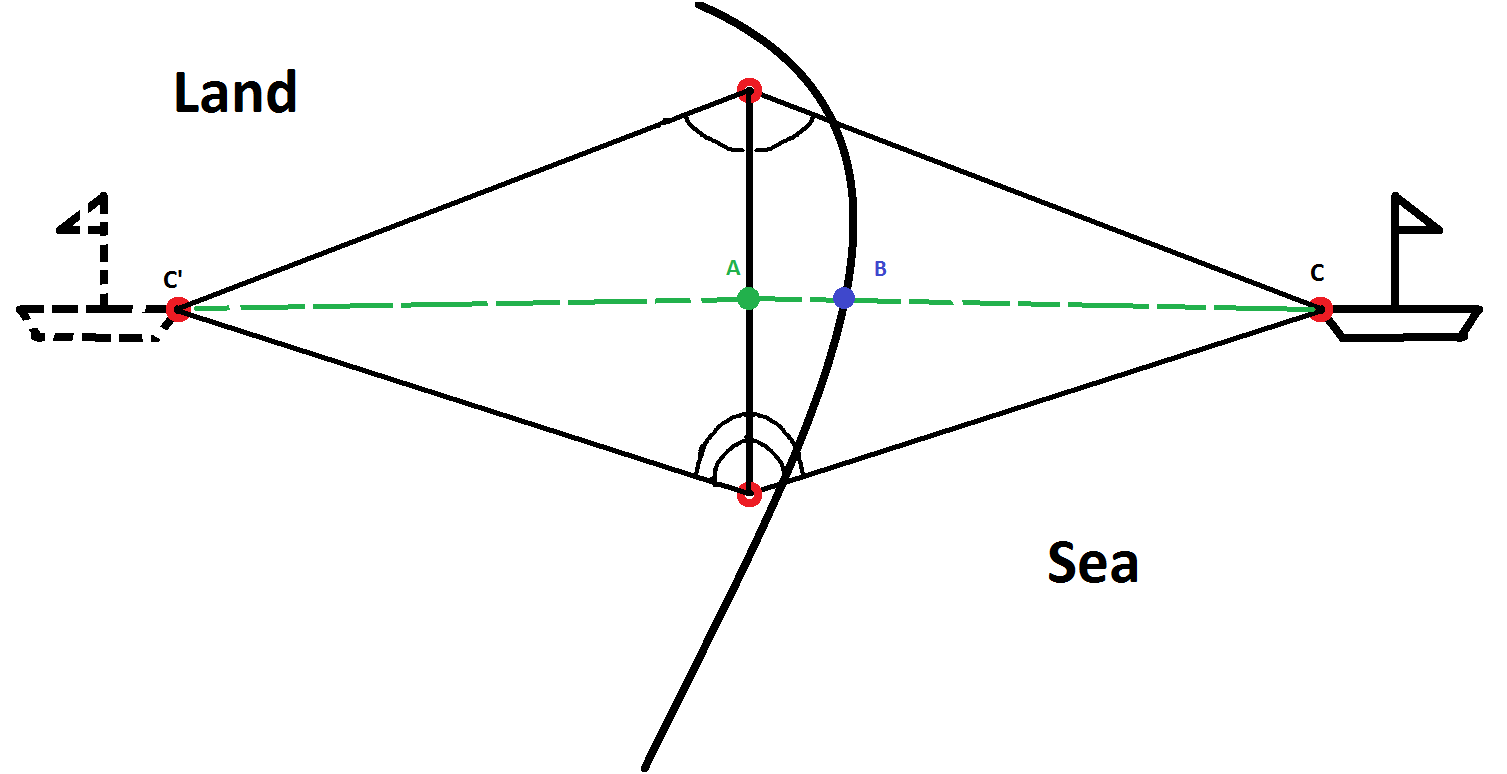
\includegraphics[width=4in]{boats.png}
\end{center}


Additionally, if he also knew that similar triangles had proportional side lengths, he could construct a small triangle with the same angle measures and measure the perpendicular distance from this to the side corresponding to the segment between the two towers.  If he did this, he would have a distance proportional to the distance along AC.    Potential sources of error are in measuring the angles, the distance between the towers, and the fact that the tower and the ship lie at 3 corners of a triangle on a sphere (more like an ellipsoid) as opposed to lying in a plane.  



\newpage
7. Eratosthenes (c. 275 B.C.), a scholar and librarian at the University at Alexandria, is credited with
calculating the circumference of the earth using the following method: Eratosthenes observed that on the
summer solstice the sun was directly overhead at noon in Syene (the present site of Aswan), while at the
same time in Alexandria, which was due north, the rays of the sun were inclined 7 12�, thus indicating
that Alexandria was 7?12� north of Syene along the earth�s surface. Using the known distance between the
two cities of 5000 stades (approximately 530 miles), he was able to approximate the circumference of the
earth. Make a diagram that depicts this method and calculate the circumference in stades and in miles.
How does this result compare to present-day estimates?

The lines in the diagram leaving Alexandria and Syene are effectively parallel.  If they actually went to the same point on the sun, they would not be parallel, but the sun is 93 million miles away, at which point they might as well be parallel.  Note that the angle labelled on the diagram is the one measured by Eratosthenes while the angle congruent to it is the same because we have ` parallel' lines.

Therefore the distance from alexandria to Syrene over the circumference is in proportion to the difference in angles over the total angle (360).  Therefore 

\begin{eqnarray*}
\frac{x}{5000} &=& \frac{360}{7.2}\\
x &=& 250000\\
&& \text{and in miles...}\\
\frac{x}{530} &=& \frac{360}{7.2}\\
x &=& 26500
\end{eqnarray*}

Modern estimates put this measurement at 24,859 miles (through the poles).  This is pretty close in my opinion.

\begin{center}
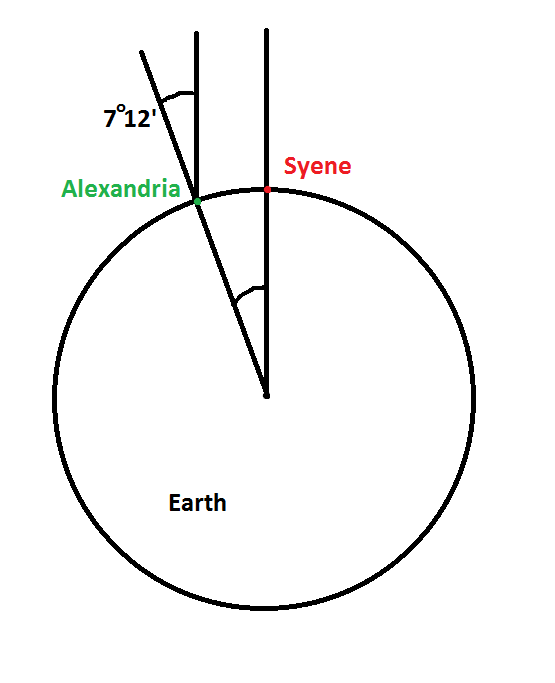
\includegraphics[width=2in]{globe.png}
\end{center}


 
 
 
 
 
 
 

\end{document}